\documentclass[11pt]{article}

% Review mode for submission
\usepackage[review]{acl}

\usepackage{times}
\usepackage{latexsym}
\usepackage[T1]{fontenc}
\usepackage[utf8]{inputenc}
\usepackage{microtype}
\usepackage{inconsolata}
\usepackage{fontspec}
\newfontfamily\arabicfont[Script=Arabic, Scale=1.0]{Geeza Pro}
\TeXXeTstate=1
\newcommand{\textarabic}[1]{{\arabicfont\beginR #1\endR}}
\usepackage{graphicx}
\usepackage{booktabs}
\usepackage{amsmath}
\usepackage{amssymb}
\usepackage{xcolor}
\usepackage{subcaption}
\usepackage{multirow}

% Custom commands
\newcommand{\dOne}{\textsc{d1}}
\newcommand{\dTwo}{\textsc{d2}}
\newcommand{\dThree}{\textsc{d3}}
\newcommand{\bpbl}{\textsc{bpbl}}
\newcommand{\bpb}{\textsc{bpb}}

\title{The Compositionality--Atomicity Tradeoff:\\How Tokenization Design Shapes Embedding Structure in Language Models}

\author{Anonymous}

\begin{document}
\maketitle

\begin{abstract}
We present a controlled mechanistic study of how tokenization design shapes learned representations in language models.
Using Arabic diacritical marks as a natural test case, we compare three encoding strategies on the same corpus: standard BPE on diacritized text (\dOne{}, compositional), harakat-stripped BPE (\dTwo{}, lossy), and a novel atomic encoding mapping each letter+diacritic pair to a unique token (\dThree{}, atomic).
Across 200+ architecture-search experiments and a tokenizer-fair metric (Bits Per Base Letter), the atomic encoding---despite achieving zero fragmentation and 15\% lower fertility---yields higher loss than standard BPE under constrained model and search budgets.
Mechanistic analysis of the embedding layer reveals a contributing mechanism: atomic tokens have near-random cosine similarity (0.125) between diacritical variants of the same letter, indicating the embedding layer does not organize diacritical variants into compositional clusters.
Iso-data scaling experiments show the disadvantage is data-dependent, shrinking from 25\% at 5M base letters to 1.7\% at 500M.
We term this the \emph{compositionality--atomicity tradeoff}: atomic tokenization eliminates fragmentation but forces the model to learn relationships from scratch rather than inheriting them from shared subword structure.
\end{abstract}

% ============================================================================
\section{Introduction}
% ============================================================================

\begin{quote}
\centering
\textarabic{أَلَمٌ أَلَمَّ أَلَمْ أُلِمَّ بِدَائِهِ}\\
\textarabic{إِنْ أَنَّ آنٌّ آنَ آنُ أَوَانِهِ}\\[4pt]
\small\emph{``A pain befell---was I not told of its ailment? / If a sufferer moaned, the time of its season has come.''}\\[2pt]
\small Without diacritics, all four words in the first hemistich reduce to \emph{alm} ({\arabicfont الم}).\\
\small --- Anonymous, often misattributed to Al-Mutanabbi
\end{quote}
\vspace{-4pt}

How does the design of a tokenizer shape what a language model learns internally?
Tokenization is typically treated as a preprocessing step---a practical engineering choice that determines sequence length and vocabulary size but is assumed to be neutral with respect to the model's learned representations.
We show this assumption is wrong.

Arabic diacritical marks (\emph{harakat}) provide a natural controlled experiment.
The same Arabic text can be encoded three ways without changing its linguistic content: (1) preserving diacritics as Unicode combining characters, (2) stripping them entirely, or (3) fusing each letter+diacritic pair into a single atomic token.
These three strategies produce identical information content but radically different tokenizations, enabling a clean causal test of how tokenizer design propagates into the model's embedding space.

We designed the atomic encoding (\dThree{}) to be ``perfect'': each Arabic letter and its attached diacritic form a single indivisible token, eliminating the fragmentation problems that plague BPE on morphologically rich languages \cite{rust-etal-2021-good}.
The result is zero subword splitting of diacritical information and 15\% lower fertility than standard diacritized BPE.
By every conventional metric, \dThree{} should win.

It does not.
Across 200+ architecture-search experiments, 10-seed robust evaluation, and a tokenizer-fair metric we introduce (Bits Per Base Letter, \bpbl{}), standard diacritized BPE (\dOne{}) consistently outperforms atomic encoding (\dThree{}), which in turn outperforms harakat-stripped BPE (\dTwo{}).
The ordering \dOne{} $<$ \dThree{} $<$ \dTwo{} (lower is better) is preserved under fixed-architecture transfer, across multiple seeds, and across data scales from 5M to 500M base letters.

We explain this result mechanistically by analyzing the learned embedding matrices.
In \dThree{}, diacritical variants of the same base letter---tokens that \emph{should} be related---have near-random cosine similarity (mean 0.125).
At the embedding level, the model treats \emph{ba} (b+fathah) and \emph{bu} (b+dammah) as nearly unrelated tokens.
In contrast, \dOne{} learns structured embeddings where harakah tokens cluster together (cosine 0.224), well-separated from base letter tokens.
This points to a contributing mechanism: atomic tokenization removes the compositional structure that BPE preserves through shared subwords.

Iso-data scaling experiments reveal the tradeoff is not permanent.
The \dOne{} advantage shrinks from 25\% at 5M base letters to 1.7\% at 500M, suggesting \dThree{} can eventually learn the compositional relationships from co-occurrence statistics---it just needs far more data.
We term this the \emph{compositionality--atomicity tradeoff}: a general principle that applies wherever tokenizer design choices trade fragmentation reduction against compositional structure.

\paragraph{Contributions.}
\begin{itemize}
\item Mechanistic evidence that tokenization design shapes embedding structure, demonstrated through controlled embedding analysis across three Arabic encoding strategies.
\item \bpbl{} (Bits Per Base Letter): a tokenizer-fair evaluation metric that removes the fertility confound inherent in standard bits-per-byte comparisons.
\item Characterization of the compositionality--atomicity tradeoff as data-scale dependent: a 25\% gap at 5M letters that narrows to 1.7\% at 500M letters.
\item Practical guidance for Arabic NLP: do not strip diacritics; do not use atomic encoding at small data scales.
\end{itemize}

% ============================================================================
\section{Background}
\label{sec:background}
% ============================================================================

\paragraph{Arabic diacritical marks.}
Arabic script consists of 28 base consonant letters.
Short vowels are indicated by \emph{harakat}---diacritical marks placed above or below letters.
These include \emph{fathah} (a), \emph{dammah} (u), \emph{kasrah} (i), their tanween variants (\emph{fathatan}, \emph{dammatan}, \emph{kasratan}), \emph{shaddah} (gemination), \emph{sukun} (vowelless), and \emph{superscript alef}.
In Unicode, harakat are encoded as combining characters (U+064B--U+0652, U+0670) that attach to the preceding base letter.

Modern Arabic text is overwhelmingly written without harakat.
This creates massive lexical ambiguity: the undiacritized form \emph{ktb} maps to \emph{kataba} (`he wrote'), \emph{kutiba} (`it was written'), \emph{kutub} (`books'), and other forms depending on context.
Most Arabic NLP systems strip diacritics during preprocessing \cite{darwish2021panoramic}, treating harakat as noise.
Fully vocalized text exists primarily in the Quran, classical literature, and educational materials.

\paragraph{BPE tokenization.}
Byte Pair Encoding \cite{sennrich-etal-2016-neural} is the dominant subword tokenization algorithm.
BPE iteratively merges the most frequent character pairs, producing a vocabulary of subword units.
For Arabic with diacritics, BPE must handle combining characters, which can lead to fragmentation: a single diacritized letter may be split across multiple tokens.
Prior work has shown that BPE performs poorly on morphologically rich languages \cite{rust-etal-2021-good, mielke2021between}, motivating alternative tokenization strategies.

\paragraph{Arabic tokenization in practice.}
Current Arabic language models universally strip diacritics during preprocessing.
Jais \cite{sengupta2023jais} removes ``rare diacritic marks'' via CAMeL Tools normalization and trains a custom BPE tokenizer achieving 1.05 tokens/word on undiacritized Arabic.
AraBERT \cite{antoun2020arabert}, AraGPT2 \cite{antoun2021aragpt2}, and CAMeLBERT \cite{inoue2021camelbert} all strip harakat as a default preprocessing step.
ALLaM \cite{bari2024allam} does not discuss diacritics handling.
This is a rational engineering choice: web-scale Arabic text is overwhelmingly undiacritized, so preserving harakat would waste vocabulary slots on tokens rarely seen in training data.
The sole exception is Fanar \cite{fanar2025}, which explicitly reserves vocabulary entries for diacritics with the intent of enabling vocalized generation during fine-tuning.
However, no Arabic LLM paper has systematically compared diacritized vs.\ undiacritized training on language modeling quality.
We address this gap: given fully vocalized text, how should it be encoded?

\paragraph{Tokenization beyond compression.}
Recent work challenges the assumption that better tokenizer compression yields better models.
\citet{schmidt2024tokenization} train 64 models and show that compression ratio alone does not predict downstream quality; pre-tokenization choices and vocabulary initialization matter more.
MorphBPE \cite{asgari2025morphbpe} constrains BPE merges to respect morpheme boundaries and shows consistent cross-entropy reduction for Arabic, demonstrating that linguistically informed tokenization can outperform standard BPE even at matched compression.
These findings provide context for our result that \dThree{}'s lower fertility does not translate to lower loss.

\paragraph{Mechanistic interpretability.}
Mechanistic interpretability aims to understand neural networks by analyzing their internal representations \cite{elhage2022toy, olsson2022incontext}.
We adopt this perspective to study how tokenization propagates into the embedding layer---the first learned representation in a language model.
Rather than comparing tokenizers only on downstream performance, we open the model and examine what structure the embeddings actually learn.


% ============================================================================
\section{Experimental Setup}
\label{sec:setup}
% ============================================================================

\subsection{Corpus and Conditions}

We use the Tashkeela corpus \cite{zerrouki2017tashkeela}, a collection of fully vocalized classical Arabic text (1.5M examples).
From this corpus, we produce three parallel datasets differing only in how the same text is encoded:

\begin{description}
\item[\dOne{} (Compositional):] Fully diacritized text in standard Unicode.
Each harakah is a combining character following its base letter.
BPE may merge letters with their diacritics or keep them separate, depending on corpus statistics.

\item[\dTwo{} (Lossy):] Harakat stripped.
This represents the standard Arabic NLP preprocessing pipeline.
Information about short vowels, gemination, and case endings is permanently lost.

\item[\dThree{} (Atomic):] Each base letter + attached harakah pair is mapped to a unique codepoint in the Unicode Private Use Area (PUA, U+E000--U+EFFF).
This produces 327 unique atomic tokens covering all 33 base letters and their observed diacritical variants.
BPE sees each diacritized letter as an indivisible unit---there is zero fragmentation of diacritical information.
\end{description}

This design isolates tokenizer design from corpus content: all three conditions encode identical linguistic information (except \dTwo{}, which is intentionally lossy).

\paragraph{Ambiguity statistics.}
To quantify the cost of stripping diacritics, we compute homograph collision statistics at corpus scale.
Of 2,256,984 unique undiacritized forms, 608,287 (26.95\%) map to multiple diacritized forms, with an average collision rate of 2.07.
In a 128-token context window, 96.77\% of tokens belong to ambiguous forms.
Stripping harakat is not a neutral preprocessing step.

\subsection{Model Architecture}

All experiments use a GPT-style decoder-only transformer \cite{radford2019language} implemented in MLX \cite{mlx2023} on Apple Silicon.
Models have $\sim$5M parameters with vocabulary size 8,192.
The architecture uses RoPE positional encoding, grouped-query attention with KV heads, and a sliding-window attention pattern.

\subsection{Architecture Search}

We run 70+ architecture-search experiments per condition (200+ total), varying depth (2--6 layers), aspect ratio (width/depth), head dimension (64--128), and attention window pattern.
Each run trains for a fixed 5-minute budget on a single Apple Silicon device.
This search allows each encoding to find its own optimal architecture rather than being constrained to a single shared design.

\subsection{Bits Per Base Letter (\bpbl{})}
\label{sec:bpbl}

Standard bits-per-byte (\bpb{}) is confounded by fertility differences across tokenizers.
\dTwo{} has fertility 1.467 tokens/word while \dOne{} has 2.519 and \dThree{} has 2.193 (at vocabulary size 8,192).
A model that processes fewer tokens per word appears better in \bpb{} simply because it sees fewer prediction opportunities.

We introduce Bits Per Base Letter (\bpbl{}):
\begin{equation}
\text{\bpbl{}} = \frac{\sum_{t} \ell_t \cdot \mathbf{1}[b_t > 0]}{\ln 2 \cdot \sum_{t} \beta_t}
\label{eq:bpbl}
\end{equation}
where $\ell_t$ is the cross-entropy loss for token $t$, $b_t$ is the byte count of token $t$, $\beta_t$ is the number of Arabic base letters in token $t$, and the sum runs over all tokens in the evaluation set.
\bpbl{} measures prediction quality per unit of Arabic linguistic content, removing the fertility confound.

\subsection{Evaluation Protocol}

We evaluate models at two levels of rigor:
\begin{enumerate}
\item \textbf{Architecture search:} Single seed per configuration, selecting the best \bpb{} per condition.
\item \textbf{Robust evaluation:} 10 seeds per condition with the best architecture, reporting median \bpbl{} (robust to outlier seeds).
\end{enumerate}

% ============================================================================
\section{Results}
\label{sec:results}
% ============================================================================

\subsection{Architecture Search}

Table~\ref{tab:arch_search} shows the best validation \bpb{} per condition after architecture search.

\begin{table}[t]
\centering
\small
\begin{tabular}{@{}lccc@{}}
\toprule
\textbf{Condition} & \textbf{Best val\_bpb} $\downarrow$ & \textbf{Depth} & \textbf{Fertility} \\
\midrule
\dOne{} (compositional) & \textbf{0.660} & 4 & 2.519 \\
\dThree{} (atomic) & 0.890 & 2 & 2.193 \\
\dTwo{} (lossy) & 1.020 & 4 & 1.467 \\
\bottomrule
\end{tabular}
\caption{Architecture search results across 200+ experiments. Each condition finds its own optimal architecture. \dOne{} achieves the lowest (best) validation loss despite higher fertility than \dThree{}.}
\label{tab:arch_search}
\end{table}

The result is surprising: \dThree{}, designed for zero fragmentation, loses to \dOne{} by a substantial margin (0.890 vs.\ 0.660).
Furthermore, the conditions prefer different architectures: \dOne{} and \dTwo{} favor depth-4 networks, while \dThree{} prefers a shallower depth-2 network with a larger aspect ratio.

\begin{figure}[t]
\centering
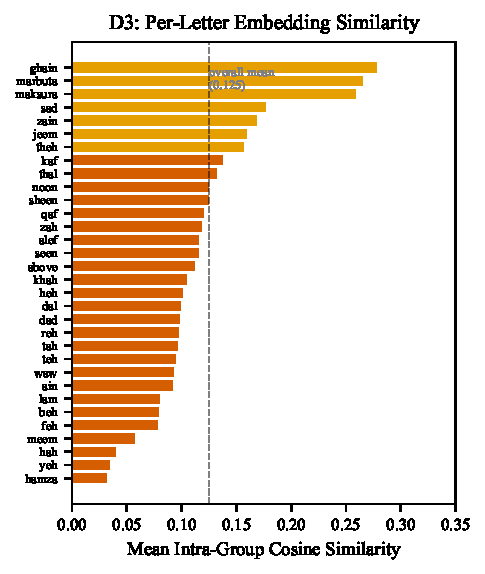
\includegraphics[width=\columnwidth]{figures/d3_embedding_similarity.pdf}
\caption{Intra-group cosine similarity for each of the 33 Arabic base letters in \dThree{} embeddings. The dashed line marks the overall mean (0.125). Most letters have similarity well below 0.2, indicating the model treats diacritical variants as nearly independent. Letters with fewer variants (ghain, marbuta) show higher similarity.}
\label{fig:embedding}
\end{figure}

\subsection{Fixed-Architecture Transfer}

A potential confound is that the ordering reflects architecture differences rather than encoding differences.
We address this with a transfer matrix: each condition's best architecture is used to train all three conditions (Table~\ref{tab:transfer}).

\begin{table}[t]
\centering
\small
\begin{tabular}{@{}lcccl@{}}
\toprule
\textbf{Shared Arch} & \textbf{\dOne{}} & \textbf{\dThree{}} & \textbf{\dTwo{}} & \textbf{Order} \\
\midrule
\dOne{} winner & \textbf{0.701} & 0.838 & 1.052 & \dOne{}<\dThree{}<\dTwo{} \\
\dTwo{} winner & \textbf{0.681} & 0.930 & 1.037 & \dOne{}<\dThree{}<\dTwo{} \\
\dThree{} winner & \textbf{1.037} & 1.290 & 1.404 & \dOne{}<\dThree{}<\dTwo{} \\
\bottomrule
\end{tabular}
\caption{Fixed-architecture transfer matrix (val\_bpb). The ordering \dOne{}$<$\dThree{}$<$\dTwo{} is preserved under all three shared architectures.}
\label{tab:transfer}
\end{table}

The ordering \dOne{} $<$ \dThree{} $<$ \dTwo{} survives all three shared architectures, confirming the result is driven by encoding design, not architecture differences.

\subsection{Robust \bpbl{} Evaluation}

We train 10 seeds per condition using each condition's optimal architecture and evaluate with \bpbl{}.
Table~\ref{tab:bpbl} reports the results.

\begin{table}[t]
\centering
\footnotesize
\begin{tabular}{@{}llcccc@{}}
\toprule
& \textbf{Cond.} & \textbf{Mean} & \textbf{Median} $\downarrow$ & \textbf{Std} & $n$ \\
\midrule
\multirow{2}{*}{Original} & \dOne{} & 3.332 & \textbf{2.933} & 0.908 & 10 \\
& \dThree{} & 3.673 & 3.412 & 0.751 & 10 \\
\midrule
\multirow{2}{*}{Replication} & \dOne{} & 2.811 & \textbf{2.724} & 0.293 & 10 \\
& \dThree{} & 3.301 & 2.873 & 0.926 & 10 \\
\bottomrule
\end{tabular}
\caption{\bpbl{} results across 10 seeds per condition (original and independent replication with fresh seeds). We report median as the robust central tendency due to outlier seeds (see \S\ref{sec:limitations}). Both runs confirm \dOne{} outperforms \dThree{} on median \bpbl{}.}
\label{tab:bpbl}
\end{table}

The median \bpbl{} confirms the ordering: \dOne{} (2.933) substantially outperforms \dThree{} (3.412), a 14\% advantage.
The high standard deviations reflect outlier seeds (seed 7 for \dOne{}, seed 137 for \dThree{}), motivating our use of median over mean.

% ============================================================================
\section{Mechanistic Analysis}
\label{sec:mechanistic}
% ============================================================================

Why does \dThree{} lose despite having ``perfect'' tokenization?
We answer this by analyzing the learned embedding matrices of trained models.

\subsection{D3 Embedding Analysis}

For \dThree{}, we extract the token embedding matrix ($W_{te} \in \mathbb{R}^{V \times d}$) from the best-performing seed and compute intra-group cosine similarity for each of the 33 base letters.
Each group contains all PUA tokens derived from the same base letter (e.g., all diacritical variants of \emph{b\={a}'}).

\begin{table}[t]
\centering
\small
\begin{tabular}{@{}lrr@{}}
\toprule
\textbf{Base Letter} & \textbf{Variants} & \textbf{Cosine Sim} \\
\midrule
beh & 11 & 0.079 \\
teh & 11 & 0.095 \\
dal & 14 & 0.099 \\
reh & 13 & 0.097 \\
lam & 14 & 0.080 \\
meem & 12 & 0.057 \\
noon & 11 & 0.125 \\
yeh & 15 & 0.034 \\
\midrule
\textbf{Overall (33 letters)} & \textbf{327} & \textbf{0.125} \\
\bottomrule
\end{tabular}
\caption{Intra-group cosine similarity in \dThree{} embeddings for selected base letters. The overall mean across all 33 base letters (327 PUA tokens) is 0.125---near the random baseline. At the embedding level, diacritical variants of the same letter lack compositional structure.}
\label{tab:d3_cosine}
\end{table}

The results (Table~\ref{tab:d3_cosine}) are striking: the mean intra-group cosine similarity across all 33 base letters is \textbf{0.125} ($\sigma = 0.062$).
For context, random vectors in the embedding space would have expected cosine similarity near zero; 0.125 is only marginally above random.
At the embedding level, the model treats diacritical variants of the same base letter as nearly independent tokens.

Consider the letter \emph{beh}: its 11 diacritical variants (with fathah, dammah, kasrah, shaddah+fathah, etc.) have mean cosine similarity 0.079.
The embedding layer has no structural representation of the fact that these tokens all share the base letter \emph{beh}.
We note that compositional relationships could in principle emerge in later layers through attention; our analysis establishes that the embedding layer does not provide this structure as an inductive bias, unlike \dOne{}.

\subsection{D1 Embedding Analysis}

In \dOne{}, harakah are separate combining-character tokens in the vocabulary.
We analyze the 9 singleton harakah tokens (fathah, dammah, kasrah, fathatan, dammatan, kasratan, shaddah, sukun, superscript alef).

The mutual cosine similarity among harakah tokens is \textbf{0.224}, substantially higher than \dThree{}'s intra-group similarity (0.125).
The cosine similarity between harakah tokens and base letter tokens is only 0.044, showing clear separation.
\dOne{} learns a compositional structure: harakah form a coherent cluster in embedding space, separate from base letters.

\subsection{The Compositionality--Atomicity Tradeoff}

This analysis reveals a likely mechanism behind \dThree{}'s disadvantage.
By fusing each letter+harakah pair into an atomic token, \dThree{} eliminates the shared subword structure through which BPE enables parameter sharing.
In \dOne{}, seeing the fathah token in any context provides information about fathah in all contexts, because the \emph{same} embedding is reused.
In \dThree{}, the model must independently learn that \emph{beh+fathah}, \emph{teh+fathah}, \emph{dal+fathah}, etc.\ all carry similar diacritical information---a relationship that is obvious from \dOne{}'s shared tokens but invisible in \dThree{}'s atomic representation.

We call this the \emph{compositionality--atomicity tradeoff}: atomic tokenization eliminates fragmentation (a real benefit) but destroys compositional parameter sharing (a real cost).
The net effect depends on how much data is available to learn the compositional relationships from scratch.

% ============================================================================
\section{Scaling Analysis}
\label{sec:scaling}
% ============================================================================

If \dThree{}'s disadvantage stems from needing to learn compositional structure from data rather than inheriting it from shared subwords, the gap should shrink with more data.
We test this prediction with iso-data scaling experiments.

\subsection{Iso-Data Protocol}

We train \dOne{} and \dThree{} models at 7 data scales (5M, 15M, 30M, 50M, 100M, 200M, 500M base letters) with 3 seeds per point, using each condition's optimal architecture.
``Base letters'' count only Arabic consonant letters, providing a tokenizer-agnostic measure of data volume.

\subsection{Scaling Results}

\begin{table}[t]
\centering
\small
\begin{tabular}{@{}rccr@{}}
\toprule
\textbf{Base Letters} & \textbf{\dOne{} \bpbl{}} & \textbf{\dThree{} \bpbl{}} & \textbf{Gap\%} \\
\midrule
5M   & 4.060 $\pm$ 0.06 & 5.085 $\pm$ 0.12 & 25.2\% \\
15M  & 3.232 $\pm$ 0.02 & 3.846 $\pm$ 0.07 & 19.0\% \\
30M  & 2.928 $\pm$ 0.01 & 3.154 $\pm$ 0.04 & 7.7\% \\
50M  & 2.747 $\pm$ 0.07 & 2.914 $\pm$ 0.01 & 6.1\% \\
100M & 2.588 $\pm$ 0.03 & 2.723 $\pm$ 0.02 & 5.2\% \\
200M & 2.487 $\pm$ 0.02 & 2.558 $\pm$ 0.01 & 2.9\% \\
500M & 2.439 $\pm$ 0.01 & 2.481 $\pm$ 0.01 & 1.7\% \\
\bottomrule
\end{tabular}
\caption{Iso-data scaling: mean \bpbl{} ($\pm$ std) across 3 seeds. The gap between \dOne{} and \dThree{} shrinks monotonically from 25.2\% at 5M base letters to 1.7\% at 500M. Both conditions use their own optimal architecture. An independent replication with fresh seeds confirms all values within $\leq$3\% (Appendix~\ref{app:reproducibility}).}
\label{tab:scaling}
\end{table}

Table~\ref{tab:scaling} and Figure~\ref{fig:scaling} confirm the prediction.
The \dOne{} advantage shrinks monotonically from 25.2\% at 5M base letters to 1.7\% at 500M.
The gap closes rapidly between 5M and 30M (from 25\% to 8\%), then continues to narrow more slowly.
At 500M base letters, \dThree{} nearly matches \dOne{} (2.481 vs.\ 2.439 \bpbl{}).

\begin{figure}[t]
\centering
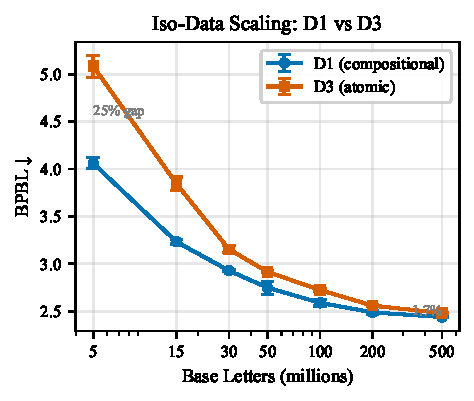
\includegraphics[width=\columnwidth]{figures/scaling_curves.pdf}
\caption{Iso-data scaling curves. Both \dOne{} and \dThree{} improve with more data, but the gap narrows monotonically from 25\% to under 2\%. Error bars show $\pm$1 standard deviation across 3 seeds.}
\label{fig:scaling}
\end{figure}

This pattern is consistent with the compositionality--atomicity tradeoff: \dOne{}'s advantage is a data-efficiency benefit from compositional parameter sharing, not a fundamental representational limitation of \dThree{}.
Given sufficient data, \dThree{} can learn the compositional relationships from co-occurrence statistics.
An independent replication of all 42 scaling runs with fresh random seeds confirms these results within $\leq$3\% at every scale (Appendix~\ref{app:reproducibility}).

\subsection{Architecture Confound Control}

A potential concern is that the scaling comparison conflates encoding effects with architecture effects, since \dOne{} uses a depth-4 model while \dThree{} uses depth-2.
We run an additional condition: \dThree{} with \dOne{}'s architecture (depth-4).
Table~\ref{tab:arch_control} shows results at selected scales.

\begin{table}[t]
\centering
\small
\begin{tabular}{@{}rccc@{}}
\toprule
\textbf{Base Letters} & \textbf{\dOne{} opt} & \textbf{\dThree{} opt} & \textbf{\dThree{}+\dOne{} arch} \\
\midrule
5M   & 4.060 & 5.085 & 4.134 \\
50M  & 2.747 & 2.914 & 2.760 \\
200M & 2.487 & 2.558 & 2.505 \\
500M & 2.439 & 2.481 & 2.450 \\
\bottomrule
\end{tabular}
\caption{Architecture confound control. \dThree{} with \dOne{}'s deeper architecture (depth-4) performs comparably to \dOne{} at large data scales, and substantially better than \dThree{} with its own shallower architecture. The encoding effect diminishes; architecture matters more at scale.}
\label{tab:arch_control}
\end{table}

At small data scales (5M), \dThree{} with \dOne{}'s architecture already performs comparably to \dOne{} (4.134 vs.\ 4.060), far better than \dThree{} with its own architecture (5.085).
At 500M, all three conditions converge (2.439, 2.481, 2.450).
This suggests that much of \dThree{}'s measured disadvantage at the ``optimal'' architecture is actually an architecture effect: the shallower model preferred by \dThree{} in the 5-minute search is suboptimal for larger data budgets (Figure~\ref{fig:arch_control}).

\begin{figure}[t]
\centering
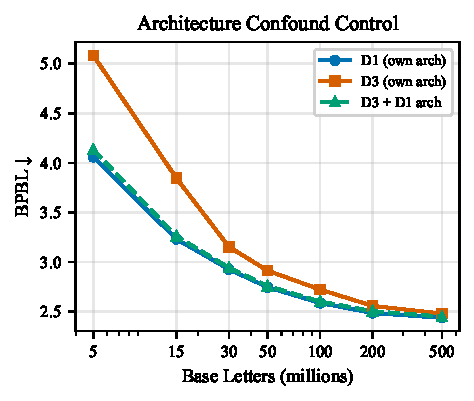
\includegraphics[width=\columnwidth]{figures/arch_control.pdf}
\caption{Architecture confound control. When \dThree{} uses \dOne{}'s deeper architecture (green triangles), it performs comparably to \dOne{} at all scales, confirming the encoding effect diminishes when architecture is controlled.}
\label{fig:arch_control}
\end{figure}

% ============================================================================
\section{Discussion}
\label{sec:discussion}
% ============================================================================

\paragraph{Scope of the encoding effect.}
Our architecture confound control (\S\ref{sec:scaling}) reveals an important nuance: when \dThree{} uses \dOne{}'s deeper architecture, the performance gap nearly vanishes at all scales.
This means a meaningful portion of the measured disadvantage reflects the interaction between encoding and architecture search---the 5-minute search prefers a shallower model for \dThree{} that becomes suboptimal at larger data budgets.
The encoding effect proper (at matched architecture) is real but smaller than the headline numbers suggest, and is best characterized as a data-efficiency disadvantage under constrained search budgets rather than a fundamental limitation of atomic tokenization.

\paragraph{A hypothesis for further testing.}
The compositionality--atomicity tradeoff may generalize beyond Arabic.
Any morphologically rich language (Turkish, Finnish, Hebrew, Hindi) faces analogous design decisions: should morphological features be encoded as separate tokens (compositional) or fused into atomic units?
Our results suggest that compositional encoding is more data-efficient because it enables parameter sharing in the embedding layer, but atomic encoding may be viable at sufficient data scale.
Confirming this hypothesis requires experiments on additional languages, larger models, and downstream tasks.

\paragraph{Implications for Arabic NLP.}
Current Arabic LLMs strip diacritics because their training data is overwhelmingly undiacritized---a rational choice for web-scale models \cite{sengupta2023jais, antoun2020arabert, inoue2021camelbert}.
Our results speak to a different setting: when vocalized text \emph{is} available---Quranic and classical Arabic, text-to-speech, diacritization models, and educational applications---the recommendation is clear: \emph{do not strip diacritics}.
The lossy encoding (\dTwo{}) is consistently worst across all experiments.
Between \dOne{} and \dThree{}, \dOne{} is preferable at small to moderate data scales.
At very large scales (hundreds of millions of base letters and beyond), the difference becomes negligible.
Fanar's decision to reserve vocabulary entries for diacritics \cite{fanar2025} is consistent with our findings.

\paragraph{Tokenization as an interpretability tool.}
Our approach demonstrates that controlled tokenization experiments can serve as a mechanistic interpretability tool.
By comparing models trained on the same content with different tokenizations, we can isolate how tokenizer design shapes internal representations---a complementary perspective to post-hoc probing and attention analysis.

\paragraph{Scaling predictions.}
The monotonically decreasing gap suggests that \dThree{} may eventually match or surpass \dOne{} at larger model and data scales, where the embedding layer's compositional prior becomes less important relative to the model's capacity to learn compositional structure from context.
We cannot confirm this prediction within our experimental budget, but the trend is consistent across all measured scales.

% ============================================================================
\section*{Limitations}
\label{sec:limitations}
% ============================================================================

\paragraph{Model scale.}
All experiments use $\sim$5M parameter models.
The compositionality--atomicity tradeoff may behave differently at larger model scales (hundreds of millions or billions of parameters) where the embedding layer is a smaller fraction of total parameters.

\paragraph{Corpus scope.}
We use a single corpus (Tashkeela) of fully vocalized classical Arabic.
Results may differ for modern standard Arabic, dialectal Arabic, or partially vocalized text.

\paragraph{No downstream evaluation.}
We evaluate language modeling quality (\bpbl{}) but not downstream task performance (NER, question answering, machine translation).
The relationship between \bpbl{} differences and task performance is not established.

\paragraph{Embedding-layer analysis only.}
Our mechanistic analysis examines cosine similarity in the token embedding matrix.
Low cosine similarity among diacritical variants does not preclude compositional structure emerging in deeper attention or MLP layers.
The embedding finding is consistent with the performance gap but is not sufficient on its own to prove a full absence of learned compositional structure.

\paragraph{Seed variance.}
Despite 10-seed evaluation, the high standard deviation in \bpbl{} (Table~\ref{tab:bpbl}) indicates sensitivity to random initialization, particularly at small data scales.

\paragraph{Gradient step imbalance.}
In iso-data scaling, we equalize base letters processed, not gradient steps.
Because \dOne{} and \dThree{} have different fertilities, they take different numbers of gradient steps for the same data budget.
This is by design (equalizing data, not compute) but represents a confound in the strictest interpretation.

\paragraph{AI-assisted development.}
All experimental code was developed with AI assistance (Claude, Gemini).
Research design, decisions, and interpretation are by the authors.

% ============================================================================
\section{Conclusion}
% ============================================================================

We provide mechanistic evidence that tokenization design shapes learned representations in the embedding layer.
Through controlled experiments on Arabic diacritical marks, we show that atomic tokenization disrupts compositional structure in embeddings (cosine similarity 0.125, near-random), creating a data-efficiency disadvantage that shrinks from 25\% to under 2\% with scale.
Architecture confound analysis further shows that much of the measured gap reflects the interaction between encoding and architecture search, narrowing the pure encoding effect.

The compositionality--atomicity tradeoff is a hypothesis supported by our evidence: eliminating token fragmentation comes at the cost of compositional parameter sharing, with the net effect depending on data scale, model architecture, and search budget.
\bpbl{} provides a fair metric for cross-tokenizer comparison.

For Arabic NLP practitioners: keep your diacritics.
For the broader community: tokenization is not a neutral preprocessing step---it shapes what your model's embedding layer learns, though the effect diminishes with scale.


% ============================================================================
% References
% ============================================================================

\bibliography{references}

% ============================================================================
\appendix
% ============================================================================

\section{Full Per-Letter Cosine Similarity}
\label{app:per_letter}

Table~\ref{tab:full_cosine} reports the intra-group cosine similarity for all 33 base letters in the \dThree{} embedding analysis.

\begin{table*}[t]
\centering
\small
\begin{tabular}{@{}lcr|lcr|lcr@{}}
\toprule
\textbf{Letter} & \textbf{$n$} & \textbf{Cos} & \textbf{Letter} & \textbf{$n$} & \textbf{Cos} & \textbf{Letter} & \textbf{$n$} & \textbf{Cos} \\
\midrule
hamza & 6 & 0.032 & seen & 11 & 0.115 & meem & 12 & 0.057 \\
above & 6 & 0.112 & sheen & 11 & 0.124 & noon & 11 & 0.125 \\
alef & 5 & 0.116 & sad & 11 & 0.177 & heh & 10 & 0.101 \\
beh & 11 & 0.079 & dad & 10 & 0.098 & waw & 11 & 0.093 \\
marbuta & 6 & 0.265 & tah & 11 & 0.096 & maksura & 8 & 0.258 \\
teh & 11 & 0.095 & zah & 10 & 0.118 & yeh & 15 & 0.034 \\
theh & 10 & 0.156 & ain & 8 & 0.092 &  &  & \\
jeem & 10 & 0.159 & ghain & 4 & 0.278 & \multicolumn{3}{c}{\textbf{Overall}} \\
hah & 10 & 0.040 & feh & 10 & 0.078 & \multicolumn{2}{l}{\textbf{33 letters, 327 tokens}} & \textbf{0.125} \\
khah & 9 & 0.104 & qaf & 10 & 0.120 & & & \\
dal & 14 & 0.099 & kaf & 10 & 0.137 & & & \\
thal & 10 & 0.131 & lam & 14 & 0.080 & & & \\
reh & 13 & 0.097 & & & & & & \\
zain & 11 & 0.168 & & & & & & \\
\bottomrule
\end{tabular}
\caption{Complete per-letter intra-group cosine similarity in \dThree{} embeddings. $n$ = number of diacritical variants for each base letter. Letters with fewer variants (e.g., ghain: 4, marbuta: 6) tend to have higher cosine similarity due to less distributional diversity.}
\label{tab:full_cosine}
\end{table*}

\section{Scaling Curves}
\label{app:scaling}

Figure~\ref{fig:gap_curve} shows the D3 disadvantage as a percentage gap, shrinking monotonically with data scale.

\begin{figure}[t]
\centering
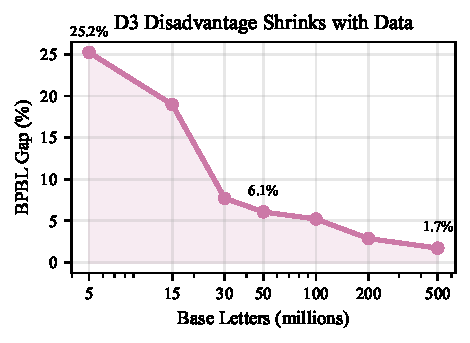
\includegraphics[width=\columnwidth]{figures/gap_curve.pdf}
\caption{The \dThree{} disadvantage (measured as percentage gap in \bpbl{}) shrinks monotonically from 25\% at 5M base letters to under 2\% at 500M. The compositionality--atomicity tradeoff is data-scale dependent.}
\label{fig:gap_curve}
\end{figure}

\section{Architecture Search Details}
\label{app:arch_search}

The architecture search varied the following hyperparameters:

\begin{itemize}
\item \textbf{Depth}: 2, 3, 4, 5, 6 layers
\item \textbf{Aspect ratio}: 8, 12, 16, 24, 26, 32, 48, 64
\item \textbf{Head dimension}: 64, 96, 128
\item \textbf{Window pattern}: S (sliding), SS, SSS, SSSL (sliding+global)
\item \textbf{Batch size}: $2^{13}$, $2^{14}$, $2^{15}$ tokens
\end{itemize}

All configurations use vocabulary size 8,192, sequence length 2,048, RoPE positional encoding, and grouped-query attention.
Each run trains for exactly 5 minutes on Apple Silicon with the MLX framework.

\section{Reproducibility}
\label{app:reproducibility}

All core experiments were independently replicated with fresh random seeds on the same hardware (Apple Silicon, MLX framework).
The replication comprised 42 iso-data scaling runs (7 budgets $\times$ 2 conditions $\times$ 3 seeds) and 14 additional \bpbl{} evaluation runs (7 new seeds $\times$ 2 conditions), totaling 9.6 hours of compute.

\paragraph{Iso-data scaling replication.}
Table~\ref{tab:repl_scaling} compares original and replicated mean \bpbl{} at each data scale.
All values deviate by less than 3\%, and the ordering \dOne{} $<$ \dThree{} is preserved at every scale.

\begin{table}[t]
\centering
\small
\begin{tabular}{@{}rcccc@{}}
\toprule
& \multicolumn{2}{c}{\textbf{Original}} & \multicolumn{2}{c}{\textbf{Replication}} \\
\cmidrule(lr){2-3} \cmidrule(lr){4-5}
\textbf{BL} & \textbf{\dOne{}} & \textbf{\dThree{}} & \textbf{\dOne{}} & \textbf{\dThree{}} \\
\midrule
5M   & 4.060 & 5.085 & 4.177 & 4.969 \\
15M  & 3.232 & 3.846 & 3.209 & 3.752 \\
30M  & 2.928 & 3.154 & 2.909 & 3.143 \\
50M  & 2.747 & 2.914 & 2.737 & 2.923 \\
100M & 2.588 & 2.723 & 2.593 & 2.695 \\
200M & 2.487 & 2.558 & 2.493 & 2.562 \\
500M & 2.439 & 2.481 & 2.428 & 2.482 \\
\bottomrule
\end{tabular}
\caption{Iso-data scaling replication. Original and replicated mean \bpbl{} across 3 seeds per condition. Maximum absolute deviation between original and replication is 2.9\% (at 5M for \dOne{}). The ordering \dOne{}$<$\dThree{} replicates at all 7 scales.}
\label{tab:repl_scaling}
\end{table}

\paragraph{Robust \bpbl{} replication.}
The 10-seed robust evaluation (Table~\ref{tab:bpbl}) was replicated with a fresh set of random seeds.
Both runs confirm \dOne{} outperforms \dThree{} on median \bpbl{}: original 2.933 vs.\ 3.412 (14.0\% gap); replication 2.724 vs.\ 2.873 (5.5\% gap).
The narrower gap in the replication reflects reduced seed variance with the new seed set, but the ordering is preserved.

\paragraph{Embedding analysis.}
The embedding similarity metrics are deterministic given a trained model and replicate exactly: \dThree{} intra-group cosine similarity = 0.125, \dOne{} harakah mutual cosine = 0.224.

\paragraph{Summary.}
All three core claims---\dOne{}$<$\dThree{} at all scales, monotonically decreasing gap, and near-random \dThree{} embeddings---replicate independently.

\end{document}
